
%\noindent
%{\bf High-Energy Primary Effects in Diboson Production}\\
In this section we classify the leading new-physics effects that can be tested
in diboson channels, showing that they can be encapsulated in four real ``high-energy primary'' (HEP) parameters~\cite{Franceschini:2017ab} .
We also assess the reach on these parameters at the HL-LHC and at future hadronic colliders, focusing in particular
on the fully leptonic $WZ$ channel that appears particularly promising.

We are interested in processes which fulfill two conditions. First, their amplitudes must receive BSM contributions that grow with $E^2$ at the leading order (i.e., $d=6$) in the EFT operator expansion. Second, the  SM amplitudes must be constant and sizable
at high energy, in such a way that, at the linear order in the EFT Wilson coefficient,  the $E^2$-growth of the BSM amplitudes
results into a $E^2$-growth of the differential cross-sections thanks to the SM-BSM interference. 
As explained in detail in Ref.~\cite{Franceschini:2017ab}, only $pp \to V_LV_L $ and $pp \to V_L h$ (see section~\ref{sec:ZHWZeft}) production
processes  enjoy quadratic energy growth at the interference level; we thus focus on these in the rest of the
section.\footnote{Notice however that promising strategies to circumvent the non-interference problem have been recently proposed \cite{Panico:2017frx,Azatov:2017kzw}, which allow for instance to ``resurrect'' interference effects in transverse vector bosons production, see also section~\ref{sec:WZtrans}.}
%\subsection{High-Energy Primary Effects}

In order to assess the leading energy behavior, it is sufficient to study the amplitude in the unbroken phase,
where the EW bosons are massless and the $G_{\rm{SM}}={\textrm{SU}}(2)_L\times{\textrm{U}}(1)_Y$ symmetry is exact.
Given that the Goldstone bosons live in the Higgs doublet $H$, together with the Higgs particle, $G_{\rm{SM}}$ implies
that the high-energy behavior of the former ones are connected with the latter. This is the reason why $V_LV_L$
and $V_Lh$ production processes, collectively denoted as $\Phi\Phi'$ in what follows, should be considered together.

Focusing our interest to the production of $\Phi\Phi'$ out of a quark $q'$ with helicity $\lambda'$ and an anti-quark ${\overline{q}}$ with helicity $\lambda$ we can restrict the form of the BSM amplitudes that interfere with SM one.
%As explained in detail in \cite{Franceschini:2017ab}  the dominance of J=1 SM amplitudes (up to corrections proportional to the light quark masses).
At order  $E^2/M^2$ in the EFT expansion the relevant BSM effects can be parametrized as corrections to the $J=1$ partial wave amplitudes~\cite{Franceschini:2017ab}, namely
\begin{equation}\label{amp0}
\delta{\mathcal{A}}\left(q^\prime_{\pm}{\overline{q}}_{\mp}\rightarrow\Phi\Phi'\right)= f^{\Phi\Phi'}_{q^\prime_{\pm}{\overline{q}}_{\mp}}(s)\sin\theta=  \frac{1}{4} A^{\Phi\Phi'}_{q^\prime_{\pm}{\overline{q}}_{\mp}}\, E^2 \sin\theta^*\,,
\end{equation}
where $\theta^*$ is the scattering angle in the $\Phi\Phi'$ center of mass, and $E=\sqrt{s}$ is the center of mass energy.

Eq.~(\ref{amp0}) shows that at the leading order in the SM EFT expansion each diboson process is sensitive at high energy to a single constant new-physics parameter $A^{\Phi\Phi'}_{q^\prime_{\pm}{\overline{q}}_{\mp}}$ for every combination of initial or final states. This can be taken real since its imaginary part does not interfere with the SM. In addition, the SM symmetry group, which is restored in the high-energy limit, as previously explained, implies  several relations among these parameters~\cite{Franceschini:2017ab}. %These relations can be found in Ref.~\cite{Franceschini:2017ab}, here we 
As a consequence, only $4$ HEP parameters are enough to parametrize the BSM effects we are interested in. This is very non-trivial from an EFT perspective, since a total of $6$ anomalous couplings coming from $d=6$ effective operators contribute to longitudinal diboson processes. These couplings can be identified as
${\delta g^Z_{uL}}$, ${\delta g^Z_{uR}}$, ${\delta g^Z_{dL}}$, ${\delta g^Z_{dR}}$, ${\delta g_1^Z}$ and ${\delta \kappa_{\gamma}}$ in the notation of Ref.~\cite{Gupta:2014rxa}.
The relations between the HEP parameters and the $4$ combinations of the low-energy primaries that produce growing-with-energy effects are reported in the third column of table~\ref{Wilsons}, while
\begin{table}[t]
\begin{center}
\begin{tabular}{c|c|c}%\hline
Amplitude& High-energy primaries& Low-energy primaries  \\\hline
\rule[-1.4em]{0pt}{3.2em}$\bar u_L d_L\to W_LZ_L,W_Lh$ & $\sqrt{2}a_q^{(3)}$ & $ \displaystyle\sqrt{2}\frac{g^2}{m_W^2}\left[c_{\theta_W}({\delta g^Z_{uL}}-{\delta g^Z_{dL}})/g-c_{\theta_W}^2{\delta g_1^Z} \right]$ \\
\hline
\rule[-.6em]{0pt}{1.7em}$\bar u_L u_L\to W_LW_L$& \multirow{ 2}{*}{$a_q^{(1)}+a_q^{(3)}$}& \multirow{ 2}{*}{$\displaystyle-\frac{2g^2}{m_W^2}\left[Y_L t^2_{\theta_W}{\delta\kappa_\gamma}+T_Z^{u_L}{\delta g_1^Z}+c_{\theta_W}{\delta g^Z_{dL}}
%-\sqrt{2}{\delta g^W_L})
 /g\right]$}\\
\rule[-.55em]{0pt}{1.45em}$\bar d_L d_L\to Z_Lh$& &\\
\hline
\rule[-.6em]{0pt}{1.7em}$\bar d_L d_L\to W_LW_L$& \multirow{ 2}{*}{$a_q^{(1)}-a_q^{(3)}$}& \multirow{ 2}{*}{$\displaystyle-\frac{2g^2}{m_W^2}\left[Y_L t^2_{\theta_W}{\delta\kappa_\gamma}+T_Z^{d_L}{\delta g_1^Z}+c_{\theta_W}{\delta g^Z_{uL}}
%+\sqrt{2}{\delta g^W_L})
/g\right]$}\\
\rule[-.55em]{0pt}{1.45em}$\bar u_L u_L\to Z_Lh$& & \\
\hline
\rule[-1.2em]{0pt}{3.em}$\bar f_R f_R\to W_LW_L,Z_Lh$& $a_{f}$& $\displaystyle-\frac{2g^2}{m_W^2}\left[Y_{f_R} t^2_{\theta_W}{\delta\kappa_\gamma}+T_Z^{f_R}{\delta g_1^Z}+c_{\theta_W}{\delta g^Z_{fR}}/g\right]$
%\\\hline
 \end{tabular}
  \caption{Parameter combinations (in the high- and in the low-energy primary bases) that control $E^2$-enhanced effects in each polarized longitudinal diboson production process. Here, $T_Z^f=T_3^f-Q_fs^2_{\theta_W}$ and $Y_{L,f_R}$ is the hypercharge of the left-handed and right-handed quark (e.g., $Y_L=1/6$).}
\label{Wilsons}
\end{center}
\end{table}
the relations between the HEP and the Wilson coefficients in the SILH basis~\cite{Giudice:2007fh} are given by
\be
 a_q^{(3)}=\frac{g^2}{M^2}(c_W+c_{HW}-c_{2W})\ ,\ \  \ \
  a_q^{(1)}=\frac{g'^2}{3M^2}(c_B+c_{HB}-c_{2B})\,, \label{a2c}
\ee
and
\be
a_u=-2a_d=4 a_q^{(1)}\,.
\label{unifersal}
\ee
These relations can also be written using  the $\hat S$, $\hat T$, $W$ and $Y$ parameters (we follow the notation of Ref.~\cite{Barbieri:2004qk}) in addition to the two anomalous  triple gauge couplings (aTGC), $\delta g_1^Z$ and  $\delta \kappa_\gamma$. We have
\be
 a_q^{(3)}=-\frac{g^2}{m_W^2}\left(c^2_{\theta_W}\delta g_1^Z+W\right)\ ,\ \  \ \
  a_q^{(1)}=\frac{g'^2}{3m_W^2}\left(\hat S-\delta\kappa_\gamma+c^2_{\theta_W} \delta g_1^Z-Y\right)\,,
\label{heptosilh}  
\ee
which  can  be useful in order to  compare HEP analyses  from  LHC  with  other experiments, such as LEP. 



In the Warsaw basis \cite{Grzadkowski:2010es}, the HEP are transparently identified with contact interactions between quarks and scalars \footnote{These relations, as well as those in  \eq{a2c}, are obtained by computing the diboson helicity amplitudes in the presence of the EFT operators, and matching with the results of the low energy primaries. See Ref.~\cite{Franceschini:2017ab} for details.}
\be
a_u=4\frac{c_R^u}{M^2}\ ,\  \ a_d=4\frac{c_R^d}{M^2}\ ,\ \  a^{(1)}_q=4\frac{c^{(1)}_L}{M^2}\ ,\ \  a^{(3)}_q=4\frac{c^{(3)}_L}{M^2}\,.
\ee


%%%%%%%%%%%%%%%%%%%%%%%%%%%%%%%%%%%%%%%%%%%%%%%%%%%%%%%%%%%%%%%%%%%%%%%%%%%%%%%%%%%%%%%%%%%%%%%%%%%%%%%%%%%%%%%%%%%%%%%%%%%%%%%%%%%%%%%%%%
%\vspace{1cm}
%\noindent
%{\bf LHC Primaries Sensitivity: The $\mathbf{WZ}$ Channel}\\
To illustrate the HL/HE-LHC reach on the high-energy primaries we focus on $WZ$ production. This channel gives access to the
$a_q^{(3)}$ primary and has a very high sensitivity to new physics~\cite{Franceschini:2017ab}. We consider the fully leptonic final state
$$
pp\to W^{\pm}Z + {\rm{jets}}\to \ell\nu\ell^{\prime}\bar{\ell}^{\prime} + {\rm{jets}} \,, \;\;\; {\rm{with}}\;\;l,l'=e,\mu\,,
$$ 
which is likely to be measured with good accuracy and can benefit from a straightforward reconstruction of the final-state
leptons and a very low reducible background~\cite{Aad:2016ett}. At the experimental level
the situation might not be too much different from the neutral Drell-Yan process, in which a measurement with $2\%$
relative systematic uncertainty of the differential cross-section was performed, with run-$1$ LHC data,
up to TeV energies~\cite{Aad:2016zzw}.
A systematic uncertainty of $5\%$ might be considered as a realistic goal for the differential cross-section measurement in the leptonic $WZ$ channel. 

The main obstacle to obtain sensitivity to new physics is the potentially large contribution of the other polarizations, which for our purposes constitute a background, since they are insensitive to the new physics parameter $a_{q}^{(3)}$. %In the $WZ$ channel these effects are automatically under control in the high-$p_T$ region and they can be further reduced by suitable selection criteria, as we will discuss later.
Due to the symmetry structure, the emission of transversely polarized $W$ and $Z$ bosons in the central rapidity region is disfavored~\cite{Franceschini:2017ab}. No suppression is instead expected for longitudinally polarized gauge bosons, therefore it is advantageous to concentrate our analysis on central scattering region, $|\cos \theta^*| \sim 0$, or, equivalently, at large $\ptv$ ($\ptv > 1\ {\rm TeV}$). We stress that other diboson processes, e.g. $pp \to WW$, do not enjoy this suppression of transverse vector boson emission, therefore are expected to be less sensitive probes of the high energy primaries. %The interested reader can find estimates of the results achievable with the other diboson channels in Ref.~\cite{Franceschini:2017ab}.

%\vspace{1cm}
%\noindent
%{\bf Analysis}\\
We now estimate the reach on $a_q^{(3)}$ based on a full NLO simulation of the $pp \to 3\ell\nu$ process, see Ref.~\cite{Franceschini:2017ab}. % to which we refer for more details.
%We perform a matched calculation that uses matrix elements computed at NLO in QCD with {\sc{MadGraph5}} with FxFx-matched %\cite{Frederix:2012ly} parton shower supplied by Pythia8~\cite{Sjostrand:2014rr}, with NNPDF~2.3~NLO parton distributions. The %signal is computed through the operator $\op_{HW}$ implemented in the NLO version of the UFO model \texttt{EWdim6}.
We consider generation-level leptons momenta, but we include an overall detector efficiency for reconstructing the three leptons that we estimate around 50\%~\cite{ATLAS:2016iqc}. We furthermore apply standard acceptance cuts on the leptons (see Table~\ref{tab:cuts}).
%\be 
%p_{T,\ell}>30 \UGeV \ ,\quad |\eta_{\ell}|<2.4\,. \label{leptonscuts}
%\ee 
The same-flavor and opposite-charge lepton pair with invariant mass closer to the $Z$ boson mass is taken as the $Z$ candidate and the remaining lepton  is taken to be the decay product of the $W$ boson. The missing transverse energy vector of the event ($\cancel{\vec{E}}_T$ ) is estimated from the generation-level transverse neutrino momentum, to which we apply a Gaussian smearing with standard deviation
$ \sigma_{{\met}_{i}}^2 = (0.5)^2 \cdot \sum_f |p_i| \cdot {\rm{GeV}}\,$.
%This approach is similar to well-tested detector performance parameterizations used e.g.~in {\sc{Delphes}}~\cite{Ovyn:2009ys,de-Favereau:2013dk}.

\begin{table}
\centering
\begin{tabular}{c|c}
acceptance cuts &
$p_{T,\ell}>30 \UGeV \ ,\quad |\eta_{\ell}|<2.4$\\
\hline
\multirow{2}{*}{analysis cuts} &
$\deltapt/p_{T,V}<%[\deltapt/p_{T,V}]_{\rm{max}}=
0.5$\\
& $|\cos \thetastar| \leq %|\cos \thetastar|_{\rm{max}}=
0.5$
\end{tabular}
\caption{List of acceptance and analysis cuts.}\label{tab:cuts}
\end{table}

In order to highlight the production of longitudinally polarized vector bosons in the central rapidity region, it is useful to eliminate events with hard real radiation, which tend to be more abundant for our background of transverse polarized gauge bosons. To tame real radiation events in a controlled way we employ a selection on the transverse momentum of the $WZ$ system, denoted by $\deltapt=|{\vec{p}}_{T,W}+{\vec{p}}_{T,Z}|\,$.\footnote{Alternatively, a jet veto might be considered, which however could lead to lower accuracy because of the experimental and theoretical uncertainties in jets reconstruction.
%The $\deltapt$ variable is instead inclusive over the hadronic final state and it does not require jet reconstruction.
See also Ref.~\cite{Campanario:2014lza} for a different approach.} We require $\deltapt$ to be smaller than $50\%$ of the transverse momentum of the gauge bosons in the event, $p_{T,V} = \min(p_{T,W}, p_{T,Z})\,$. We also impose a cut on the scattering angle in the $WZ$ center of mass frame
$|\cos \thetastar| \leq  0.5\,$. The cuts are summarized in Table~\ref{tab:cuts}.



The kinematical variables described so far allow us to determine $p_{T,Z}$ and $p_{T,W}$, and in turn $p_{T,V}$ and $p_{T,VV}$, used to construct the binned distribution and for the selection cuts. In order to extract $|\cos \thetastar|$ the neutrino rapidity is reconstructed by the standard technique of imposing the invariant mass of the neutrino plus lepton system to be as close as possible to the physical $W$ boson mass.
A twofold ambiguity in the reconstruction is resolved by imposing the $|\cos \thetastar|$ cut on both solutions, i.e.~by retaining for the analysis only events such that both the possible neutrino configurations satisfy the selection criteria.

We study the $3$ collider energy options that correspond to the LHC ($14$~TeV), to the High-Energy LHC (HE-LHC, $27$~TeV) and to the FCC-hh ($100$~TeV). In each case we consider suitably designed $p_{T,V}$ bins, namely 
\begin{eqnarray}\label{finalbins}
{\textrm{LHC\hspace{-10pt}}}&{\textrm{:}}& p_{T,V}\in\{100,150,220,300,500,750,1200 \}\,,\\
{\textrm{HE-LHC\hspace{-10pt}}}&{\textrm{:}}& p_{T,V}\in\{150,220,300,500,750,1200, 1800 \}\,,\nonumber\\
{\textrm{FCC\hspace{-10pt}}}&{\textrm{:}}& p_{T,V}\in\{220,300,500,750,1200, 1800, 2400 \}\,.\nonumber
\end{eqnarray}
The binning is chosen such as to cover the kinematical regime that is accessible at each collider and it is taken as fine as possible in order to maximize the BSM sensitivity. On the other hand, a minimum bins size $\Delta p_{T,V}/ p_{T,V}\gtrsim30\%$ is required in order to avoid a degradation of the accuracy due to the $p_{T,V}$ resolution.



The predicted cross-sections are used to construct the $\chi^2$, under the assumption that observations  agree with the SM, and are eventually used to derive $95\%$~CL bounds on $a_q^{(3)}$. The uncertainties in each bin are the sum in quadrature of the statistical error, obtained from the SM expected events yield, and of a systematical component (uncorrelated across bins) which we take as a fixed fraction ($\delta_{\textrm{syst}}$) of the SM expectations. With this procedure we obtain, for different collider energies and luminosities and for $\delta_{\textrm{syst}}=5\%$
\begin{eqnarray}
%{\textrm{LHC, }} 300\,{\textrm{fb}}^{-1}\hspace{-10pt} & {\textrm{:}} & a^{(3)}_q  \in  [-1.4, 0.9] \,10^{-1}\,\UTeV^{-2}\nonumber\\
{\textrm{HL-LHC, }} 3\,{\textrm{ab}}^{-1}\hspace{-10pt} & {\textrm{:}} & a^{(3)}_q  \in  [-4.9, 3.9] \,10^{-2}\,\UTeV^{-2}\nonumber\\
{\textrm{HE-LHC, }} 10\,{\textrm{ab}}^{-1}\hspace{-10pt} & {\textrm{:}} & a^{(3)}_q  \in  [-1.6, 1.3] \,10^{-2}\,\UTeV^{-2}\nonumber\\
{\textrm{FCC-hh, }} 20\,{\textrm{ab}}^{-1}\hspace{-10pt} & {\textrm{:}} & a^{(3)}_q  \in  [-7.3, 5.7] \,10^{-3}\,\UTeV^{-2}
\label{boundsf}
\end{eqnarray}
We see that the HE-LHC will improve the HL-LHC reach by a factor of $3$, while a gain of nearly one order of magnitude would be possible with the FCC-hh collider. The FCC-hh reach is comparable with the one of CLIC, as extracted from the analysis in Ref.~\cite{Ellis:2017kfi}.
 
%Notice that the choice $\delta_{\textrm{syst}}=5\%$ is not based on a careful assessment of the experimental systematical uncertainties and of the theory errors on the SM predictions. At the experimental level, we argued that $\delta_{\textrm{syst}}=5\%$ could be a reasonable target, based on analogies with other purely leptonic final states. For what concerns theory, parton luminosity uncertainties are well below $5\%$ in the energy range of interest and that the scale variations in the NLO calculation are of order $5\%$. Scale variations were estimated using MCFM~8.0~\cite{Boughezal:2016ek,Campbell:2011fp} by varying renormalization and factorization scale as $\mu_{R}=\mu_{F}=2^{\pm 1} (m_{W}+m_{Z})$. We will discuss later in this section how a larger or a smaller value of $\delta_{\textrm{syst}}$ would affect the reach.
 
The results of \eq{boundsf}  rely on BSM cross-section predictions obtained by integrating up to very high center of mass energies, formally up to the collider threshold. Therefore these limits assume that the description of the underlying BSM model offered by the EFT is trustable in the whole relevant kinematical regime, i.e.~that the cutoff $M$ of the BSM EFT is high enough. We quantify how large $M$ concretely needs to be for our results to hold by studying~\cite{Racco:2015dxa,Pobbe:2017wrj,Biekoetter:2014jwa} how the limit deteriorates if only events with low $WZ$ invariant mass, $m_{\textsc{wz}}<m_{\textsc{wz}}^{\rm{max}}$ are employed. This obviously ensures that the limit is consistently set within the range of validity of the EFT provided the EFT cutoff $M$ is below $m_{\textsc{wz}}^{\rm{max}}$. The results are reported in figure~\ref{fig:bounds_future}. Since the $95\%$~CL interval is nearly symmetric around the origin only the upper limit is reported in the figure for shortness.

\begin{figure}[t]
\centering
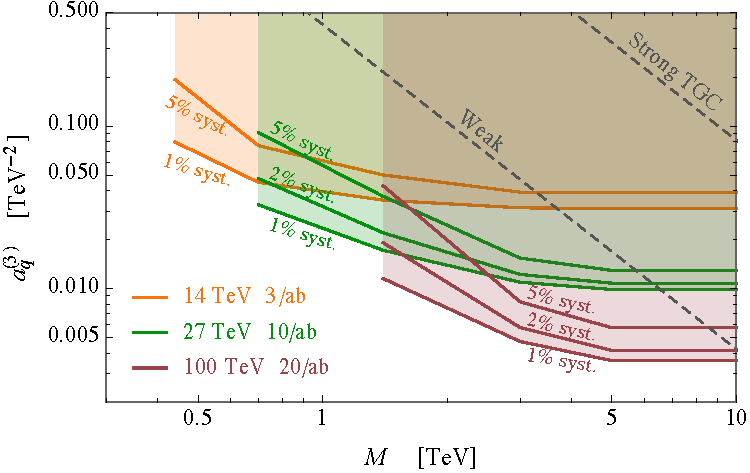
\includegraphics[width=0.7\textwidth]{\main/section4/plots/MoneyPlotCombined}
\caption{Expected $95\%$ CL bounds from fully leptonic $WZ$ on the high-energy primary parameter $a^{(3)}_q$ as a function of the new physics scale $M$. The plots reports the results for the HL-LHC (orange lines), HE-LHC (green lines) and FCC-hh (brown lines) for different
values of the systematic uncertainties.} 
\label{fig:bounds_future}
\end{figure}

Several conclusions can be drawn from figure~\ref{fig:bounds_future}. First of all we see that the reach saturates for $m_{\textsc{wz}}^{\rm{max}}$ below around $1.5$~TeV at the HL-LHC if the systematic uncertainties are low, meaning that the limits obtained without $m_{\textsc{wz}}$ cut apply to theories with cutoff $M$ above that threshold.  The threshold grows to around $3$ and $4$~TeV at the HE-LHC and at the FCC-hh, respectively. The figures show that $\delta_{\textrm{syst}}=5\%$ is sufficient to probe ``Weak'' theories in all cases, but it also shows that the impact of larger or smaller uncertainties on the reach can be significant. Systematic errors at the $\delta_{\textrm{syst}}=5\%$ level already make an appreciable difference with respect to $\delta_{\textrm{syst}}=1\%$. This is due to the fact that the low-$p_{T,V}$ bins have small statistical error and the reach in those bins benefits from lower systematics. The effect is even more pronounced at the HE-LHC and at the FCC-hh, where even with $\delta_{\textrm{syst}}=2\%$ the reach deteriorates significantly with respect the ideal case $\delta_{\textrm{syst}}=1\%$. The fact that more accurate measurements would improve the reach of future colliders is an element that should be taken into account in the design of the corresponding detectors.

